\documentclass[paper=a4,11pt,parskip=half,toc=listof]{scrartcl}
\usepackage{etoolbox}

% % % % % LANGUAGE % % % %
\newtoggle{german} % Make your choic here
%\togglefalse{german} % English
\toggletrue{german} % German
% % % % % \LANGUAGE % % % %

\usepackage[utf8]{inputenc} % input files werden als utf8 interpretiert
\usepackage[T1]{fontenc} % die schriftart wird mit T1 codiert (will man haben)

\iftoggle{german}{
\usepackage[ngerman]{babel} % Deutsche Sprachanpassungen
\usepackage[german=quotes]{csquotes} % Anfuehrungszeichen
}{
\usepackage[english]{babel} % Deutsche Sprachanpassungen
\usepackage[english=american]{csquotes} % Anfuehrungszeichen
}

\usepackage{scrpage2}
\usepackage{listings}
\lstset{
  breaklines=true,
  frame=single,
  basicstyle=\footnotesize\ttfamily
}
\usepackage{color}
\usepackage{textcomp}
\usepackage{mathtools}
\usepackage{nicefrac}
\usepackage{amsmath}
\usepackage{cite}
\usepackage{graphicx}
\usepackage{longtable}
\usepackage{float}
\usepackage{setspace}
\usepackage{url}
\usepackage{tabularx}
\usepackage{makecell}
\usepackage{multirow}
\usepackage{wrapfig}
\usepackage{pdfpages}
\usepackage{amssymb}
\usepackage{graphicx}
\usepackage[font=small]{caption} % very thin
\usepackage{subcaption}
\usepackage{picinpar}

% No footnotes on the next page please
\interfootnotelinepenalty=10000

%opening
\def\ThesisTitle{My awesome title}
\def\ThesisAuthor{John Doe}
\def\ThesisLocation{Sankt Augustin}
\def\ThesisType{Master}
\def\ThesisPubDate{\today} % Change here to the date you are going to print your thesis
\def\ThesisFirstSupervisor{Prof. Dr. Karl Jonas}
\def\ThesisSecondSupervisor{Prof. Dr. Kerstin Uhde}
\def\ThesisExternalSupervisor{Dr. Mathias Kretschmer}
\def\ThesisExternalCompany{Fraunhofer FOKUS}
\def\ThesisSubject{}


\usepackage{todonotes}
\usepackage{pdfpages} % directly include pdf pages
\usepackage{algorithmic} % pseudo-code
\usepackage{blindtext}
\usepackage[printonlyused]{acronym} 
%\usepackage[firstpage]{draftwatermark} % comment in if you submit a draf. 
\DeclarePairedDelimiter{\ceil}{\lceil}{\rceil}

% new types for a table
\newcolumntype{C}[1]{>{\centering\arraybackslash}p{#1}}
\newcommand{\specialcell}[2][l]{%
  \begin{tabular}[#1]{@{}c@{}}#2\end{tabular}}
  



%%%% Font %%%%
% \usepackage{times} % times in text
\usepackage{mathptmx} % times in math
\usepackage{setspace} \onehalfspacing %
\usepackage[paper=a4paper]{geometry}
\setlength{\parindent}{0pt} % no indent
\setlength{\headheight}{1.1\baselineskip}
\setcounter{tocdepth}{4}
\setcounter{secnumdepth}{4}
%%%% Font %%%%

%%%% footer and header %%%%
\usepackage{scrpage2}%
\pagestyle{scrheadings}%  S
\clearscrheadfoot% 
\setheadwidth{text}%
\automark{section}% 
\ohead{\textbf{\pagemark}}
\renewcommand{\sectionmark}[1]{\markright{\ #1}} 
\ihead{\textbf{\rightmark}}
\setheadsepline{0.5pt}
%%%% \footer and header %%%%

\newcolumntype{Y}{>{\centering\arraybackslash}X}




\usepackage[bookmarks=true]{hyperref}
\hypersetup{
    unicode=false,          % non-Latin characters in Acrobat’s bookmarks
    pdftoolbar=true,        % show Acrobat’s toolbar?
    pdfmenubar=true,        % show Acrobat’s menu?
    pdffitwindow=false,     % window fit to page when opened
    pdfstartview={FitH},    % fits the width of the page to the window
    pdftitle={\ThesisTitle},    % title
    pdfauthor={\ThesisAuthor},     % author
    pdfsubject={\ThesisTitle},   % subject of the document
    pdfcreator={\ThesisAuthor},   % creator of the document
    pdfproducer={\ThesisAuthor}, % producer of the document
    pdfkeywords={802.11} {DCF} {long-distance} {modeling}, % list of keywords
    pdfnewwindow=true,      % links in new window
    colorlinks=false,       % false: boxed links; true: colored links
    linkcolor=red,          % color of internal links (change box color with linkbordercolor)
    citecolor=green,        % color of links to bibliography
    filecolor=magenta,      % color of file links
    urlcolor=cyan           % color of external links
}


\begin{document}
%%%%%%%%%%%%%%%%%%%%% Startseite %%%%%%%%%%%%%%%%%%%%%%%%%%%
\begin{titlepage}
\begin{minipage}[t]{0.5\textwidth}
\begin{Large}
    \begin{flushleft}
      \hspace{1cm} \makebox[3cm][c]{
\includegraphics[height=8ex]{./logos/logo_hm.png} \vspace{1.8cm}}
    \end{flushleft}
\end{Large}
\end{minipage}
%\begin{minipage}[t]{0.5\textwidth}
% Can be an external company! Play with thge vspaces to look nice.
%\begin{Large}
%    \begin{flushright}
%     \makebox[3cm][c]{
\includegraphics[height=8ex]{./logos/logo_hbrs.png} \vspace{1.8cm}} \hspace{1cm}
%    \end{flushright}
%\end{Large}
%\end{minipage}
\vspace{0.07\textheight}
\begin{center}
 \begin{Large} \textbf{\ThesisUniversityCourse} \end{Large}\\
 \vspace{1em}
 \begin{Large} \textbf{-- \ThesisSemester --} \end{Large}\\
 \vspace{2em}
 \begin{Huge} \begin{spacing}{1.3} \textbf{\ThesisTitle} \end{spacing} \end{Huge}
 \vspace{2em}
 \iftoggle{german}{%
  \begin{Large}\textbf{von} \end{Large}\\
 }
 {%
  \begin{Large}\textbf{by} \end{Large}\\
 }
 \vspace{2em}
 \begin{Large}\textbf{\ThesisAuthor}\end{Large}\\
\end{center}
%\vspace{0.100\textheight}
\begin{large}
\begin{flushleft}
% use packages: array
\vfill
\iftoggle{german}{%
\begin{tabularx}{\textwidth}{lX}
 Erstprüfer: & \ThesisFirstSupervisor \\
 Zweitprüfer: & \ThesisSecondSupervisor \\
 Betreuer: & \ThesisExternalSupervisor \\
 Unternehmen ~ & \ThesisExternalCompany \\ % Comment out if not needed
 Eingereicht am: & \ThesisPubDate % Comment out if not needed
\end{tabularx}
}
{%
\begin{tabularx}{\textwidth}{lX}
 First supervisor: & \ThesisFirstSupervisor \\
 Second supervisor: & \ThesisSecondSupervisor \\
 External supervisor: & \ThesisExternalSupervisor \\
 External company ~ & \ThesisExternalCompany \\ % Comment out if not needed
 Handed in: & \ThesisPubDate % Comment out if not needed
\end{tabularx}
}




\end{flushleft}
\end{large}
\end{titlepage}

\newgeometry{top=4cm, bottom=3cm, left=4.5cm, right=3cm}

\thispagestyle{empty}
\begin{center}
\huge \textbf{Erklärung}
\end{center}
\vspace{5cm}
Hiermit erkläre ich an Eides Statt, dass ich die vorliegende Arbeit selbst angefertigt habe; 
die aus fremden Quellen direkt oder indirekt übernommenen Gedanken sind als solche kenntlich 
gemacht. Die Arbeit wurde bisher keiner Prüfungsbehörde vorgelegt und auch noch nicht veröffentlicht.
\vspace*{8cm}
\begin{table}[h!]
 \centering
 \begin{tabular}{cc}
  Bonn, den \iftoggle{german}{\ThesisPubDate}{\germandate{\ThesisPubDate}} & \hspace*{6cm} \\
  \midrule
  Datum								& Unterschrift\\
 \end{tabular}
\end{table}
\pagenumbering{Roman} % Big roman numbers until the text begins
\addtocontents{toc}{\protect\markright{}}

\setcounter{page}{3} % inhaltsverzeichnis beginnt auf seite 3
\begin{spacing}{1.14} % set me to something nice when ready
\tableofcontents
\end{spacing}

\clearpage{}
\listoftables % add list of tables
\clearpage{}
\listoffigures % add list of figures 
\clearpage{}
%\section*{List of abbreviations}
%\sectionmark{List of abbreviations}
%\addcontentsline{toc}{section}{List of Abbreviations}
\begin{acronym}[CSMA/CD]
\setlength{\itemsep}{-\parsep}
\acro{AP}{Access Point}
\acro{AIFS}{Arbitration Interframe Space}
\acro{AC}{Access Category}
\acro{ACK}{acknowledgement}
\acro{AS}{Autonomous System}
\acro{BER}{Bit Error Rate}
\acro{CW}{Contention Window}
\acro{CSMA/CD}{Carrier Sense Multiple Access/Collision Detection}
\acro{CSMA/CA}{Carrier Sense Multiple Access/Collision Avoidance}
\acro{CSMA}{Carrier Sense Multiple Access}
\acro{CPU}{Central Processing Unit}
\acro{DCF}{Distributed Coordination Function}
\acro{DIFS}{DCF Interframe Space}
\acro{SIFS}{Short Interframe Space}
\acro{DHCP}{Dynamic Host Configuration Protocol}
\acro{DSSS}{Direct-Sequence Spread Spectrum}
\acro{EDCF}{Enhanced Distributed Coordination Function}
\acro{EDCA}{Enhanced Distributed Coordination Access}
\acro{EIFS}{Extended Interframe Space}
\acro{EIRP}{Equivalent isotropically radiated power}
\acro{FCS}{Frame Check Sequence}
\acro{FEC}{Forward Error Correction}
\acro{FIFO}{First-In-First-Out}
\acro{FSPL}{Free-space path loss}
\acro{FSL}{Free-Space Loss}
\acro{GPS}{Global Positioning System}
\acro{HCF}{Hybrid Coordination Function}
\acro{HOL}{Head-of-line}
\acro{HCCA}{HCF controlled channel access}
\acro{IBSS}{Independent Basic Service Set}
\acro{ISM}{Industrial, Scientific and Medical}
\acro{IEEE}{Institute of Electrical and Electronics Engineers}
\acro{IETF}{Internet Engineering Task Force}
\acro{IP}{Internet Protocol}
\acro{IFS}{Interframe Space}
\acro{IPv4}{Internet Protocol}
\acro{MAC}{Media Access Control}
\acro{IPv6}{Internet Protocol, Version 6}
\acro{ISP}{Internet Service Provider}
\acro{LoS}{Line of Sight}
\acro{LGI}{Long Guard Interval}
\acro{MIMO}{Multiple Input Multiple Output}
\acro{MTU}{Maximum Transmission Unit}
\acro{MCS}{Modulation and Coding Scheme}
\acro{MSDU}{MAC Service Data Unit}
\acro{MPLS}{Multiprotocol Label Switching}
\acro{MPDU}{MAC Protocol Data Unit}
\acro{NAV}{Network Allocation Vector}
\acro{NTP}{Network Time Protocol Unit}
\acro{OSI}{Open Systems Interconnection}
\acro{OFDM}{Orthogonal Frequency-Division Multiplexing}
\acro{QoS}{Quality of Service}
\acro{RSSI}{Received Signal Strength Indication}
\acro{SGI}{Short Guard Intervall}
\acro{SNR}{Signal-to-noise ratio}
\acro{PER}{Packet Error Rate}
\acro{PPDU}{Physical Protocol Data Unit}
\acro{ToS}{Type of Service}
\acro{TCP}{Transmission Control Protocol}
\acro{TDMA}{Time Division Multiple Access}
\acro{TSFT}{Time Synchronization Function Timer}
\acro{TXOP}{Transmit opportunity}
\acro{PCF}{Point Coordination Function}
\acro{PLCP}{Physical Layer Convergence Protocol}
\acro{PTP}{Precision Time Protocol}
\acro{UDP}{User Datagram Protocol}
\acro{UP}{User Priorities}
\acro{VoIP}{Voice over Internet Protocol}
\acro{WiBACK}{Wireless Back-Haul}
\acro{WiLD}{WiFi based Long Distance networks}
\acro{WiMAX}{Worldwide Interoperability for Microwave Access}
\acro{WLAN}{Wireless Local Area Network}
\acro{WMN}{Wireless Mesh Network}
\end{acronym}
 % include the acronym thing
\clearpage{}

%%%%%%%%%%%%%%%%%%%%% Startseite %%%%%%%%%%%%%%%%%%%%%%%%%%%
\setcounter{tocdepth}{4} 
\setcounter{secnumdepth}{4}

\pagenumbering{arabic} % arabic numbers for the main part

% Here the chapters are included
\section{Introduction}
This is the introduction of an awesome thesis. In the following are some usefull examples.

\subsection{A table}
Here is a cool table \ref{tab:soa-edca} you can reference it in the text. 
\begin{table}[htbp]
\setlength{\tabcolsep}{.16667em}
\caption{State of the art of analytical models for the EDCA}
\begin{tabularx}{\textwidth}{ |p{2cm}||c|c||c|c||c|c||c|Y| }
\hline
& \multicolumn{2}{c||}{Assumptions} & \multicolumn{2}{c||}{Metric} & \multicolumn{2}{c||}{Validation} & \multicolumn{2}{c|}{Origin} \\
\cline{2-9}
\multirow{-2}{*}{Publication} & \small Saturated & \small Ideal channel & \small Throughput & \small Delay & \small Simul. & \small Experim. & \small Cali \quad & \small Bianchi \\
\hline
\cite{Robinson2004}& \checkmark & \checkmark & \checkmark &  & \checkmark &  & & \checkmark \\
\hline
\cite{Mangold2003}& \checkmark & \checkmark & \checkmark &  & \checkmark &  & & \checkmark \\
\hline
\cite{Kong2004}& \checkmark & \checkmark & \checkmark & \checkmark & \checkmark &  & & \checkmark \\
\hline
\cite{Engelstad2005}&  &  & \checkmark & \checkmark & \checkmark &  & & \checkmark \\
\hline
\cite{Banchs2005}& \checkmark & \checkmark &  &  & \checkmark &  & \checkmark &  \\
\hline
\end{tabularx}
\label{tab:soa-edca}
\end{table}

\subsection{A figure}
Here is a cool figure. It is even a subfigure.

\begin{figure}[h!]
	\centering
	\subfigure[Basic access \citep{ieee-802.11-2012}]{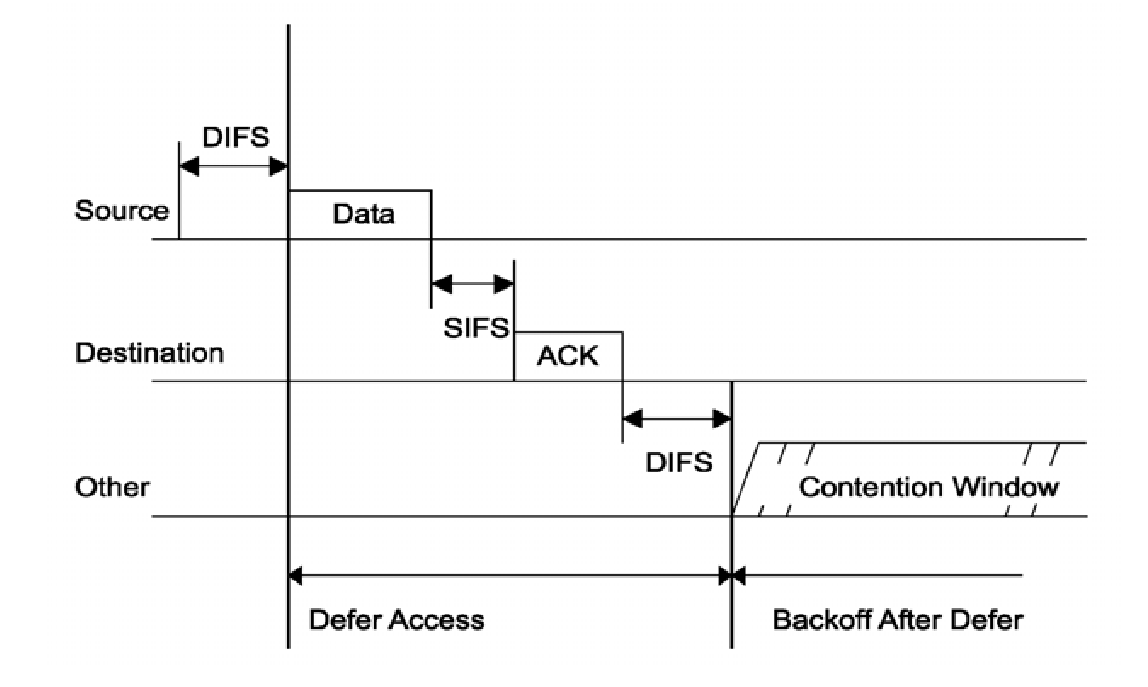
\includegraphics[width=0.39\textwidth]{figures/dcf-basic-access.png}}
	\subfigure[Back-off procedure \citep{ieee-802.11-2012}]{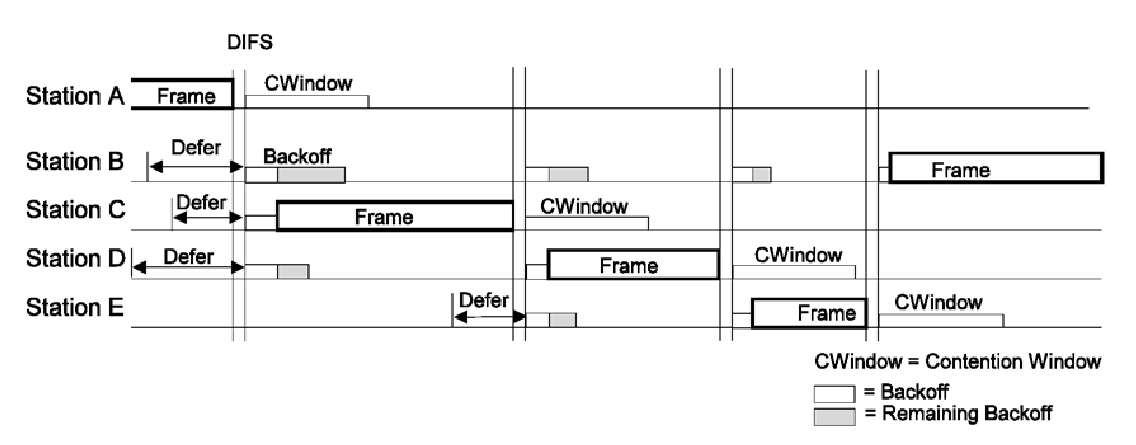
\includegraphics[width=0.59\textwidth]{figures/dcf-backoff.png}}
	\caption{\acf{DCF}}
	\label{fig:lime-sample}
\end{figure}

Um eine Seite zu zitieren: $\backslash$citep[p. 838]\{ieee-802.11-2012\} $\Rightarrow$ \citep[p. 838]{ieee-802.11-2012}

% One paragrah for one idea!
\blindtext

\blindtext

\blindtext % introduction  

% choose your type of citation here
%\bibliographystyle{plainnat} % author and year
%\bibliographystyle{amsalpha} % author and year short
\bibliographystyle{alphaabbr} % author short and year
%\bibliographystyle{alpha} % author and year
%\bibliographystyle{plain} % only numbers
%\bibliographystyle{unibonn_ay} % a special file used for the uni bonn
\singlespacing % bibliography with single spacing
% \nocite{*} % print all references in bib file regardless of citing
\bibliography{references}

% Start of the appendix
\appendix 
% The appendix is a chapter
\iftoggle{german}{
\section{Anhang}
}{
\section{Appendix}
}
This is the appendix

\end{document}